\pdfoutput=1
\documentclass[11pt,a4paper]{article}
\usepackage{abhijit-research}
\renewcommand{\PaperCode}{P10}
\renewcommand{\PaperKind}{RESEARCH PAPER}
\renewcommand{\PaperVersion}{VERSION 1.0}
\renewcommand{\PaperDate}{AUGUST 2026}
\renewcommand{\PaperTitle}{Future-Relevant Representation Disagreement}
\renewcommand{\PaperSubtitle}{Chronological Feature Restoration}
\renewcommand{\PaperFullTitle}{Future-Relevant Representation Disagreement and Chronological Feature Restoration}
\renewcommand{\PaperShortTitle}{Representation Disagreement}
\renewcommand{\PaperKeywords}{representation disagreement; chronological validation; feature restoration; ensemble routing; predictive sufficiency}
\renewcommand{\PaperClassification}{Raw environmental-file audits are independently reproduced. Downstream environmental and static-representation results are source-reported because the complete original constructors and static dataset are not in the supplied local archive.}
\renewcommand{\PaperCitation}{Singh, Abhijit. 2026. \textit{Future-Relevant Representation Disagreement and Chronological Feature Restoration}. Research manuscript, version 1.0.}
\begin{document}
\MakeResearchTitle
\MakeResearchContents
\MakeResearchAbstract{%
Two held-out studies test whether differences discarded by current-state compression remain relevant for later continuation. In a 1,797-sample, 64-coordinate corpus, three independently generated representations attain 90.74--92.96 percent exact whole-object continuation, while a relation-aware router using only child status, agreement, and prior contact performance reaches 97.78 percent, equal to the empirical oracle ceiling. A context-dependent return separately reaches 99.768 percent accuracy on admitted coordinates. In a 13-channel hourly environmental chronology, three constructors omit the same coordinate; four chronological contact blocks support restoration, and untouched-future performance improves from 72.0836 to 74.7125 percent per coordinate and from 3.7540 to 7.2492 percent for exact vectors. Negative controls reject indiscriminate higher arity and deeper history.
}
\section{Common experimental question}
Both studies test whether a distinction discarded by present-state compression remains relevant to future continuation. A candidate coordinate or relation is omitted, evaluated on chronological or held-out contact data, and restored only if it changes later prediction. The final test set remains untouched until the representation is frozen.

For current representation $Z$, candidate residual $A$, future target $Y^+$, and frozen loss $\mathcal R$, define
\begin{equation}
\Delta_{\rm fut}(A\mid Z)=\mathcal R(Y^+\mid Z)-\mathcal R(Y^+\mid Z,A).
\end{equation}
Positive held-out gain licenses promotion for the declared task; it does not imply that every extra feature should be retained.

\part{Study I: relation among independent representations}
\section{Design}
The frozen corpus contains 1,797 samples and 64 output coordinates. Three representations are generated independently before a 270-case untouched holdout is opened. Their exact whole-object continuation rates are
\begin{equation}
92.96\%,\qquad90.74\%,\qquad91.48\%.
\end{equation}
A fourth model receives only child status, agreement/disagreement relations, and performance on prior contact cases. It does not receive the semantic class labels or virgin answers.

\section{Result}
The relation-aware model reaches
\begin{equation}
\boxed{264/270=97.78\%}
\end{equation}
exact whole-object continuation, equal to the empirical oracle ceiling of the available child repertoire. Removing the agreement relation lowers the result to $97.41\%$ and produces an additional failure and two additional unknowns.

Higher relation arity did not repair cases in which all three child representations failed: the tested ternary constructor solved $0/6$ such cases. Agreement is useful only when at least one constituent representation already carries relevant future information.

\section{Context-dependent output formation}
A second experiment chooses an output coordinate set before answer comparison. Across all 270 cases the return is nonempty, with mean size $7.985$ of eight coordinates. Admitted-coordinate accuracy is
\begin{equation}
99.768\%,
\end{equation}
and whole-return correctness is
\begin{equation}
98.52\%.
\end{equation}
These are different answer objects and must not be pooled with the $97.78\%$ whole-object routing metric.

\part{Study II: chronological environmental record}
\section{Raw data audit}
The supplied semicolon-delimited file contains:
\begin{table}[H]\centering
\caption{Independent raw-file audit.}
\begin{tabular}{lr}
\toprule
raw rows & 9471\\
blank trailer rows & 114\\
nonblank hourly rows & 9357\\
completely empty columns & 2\\
numeric channels & 13\\
missing sentinel cells ($-200$) & 16701\\
rows complete on all channels & 827\\
\bottomrule
\end{tabular}
\end{table}
The nonblank timestamps are strictly hourly from 10 March 2004 18:00 to 4 April 2005 14:00.

\begin{figure}[H]\centering
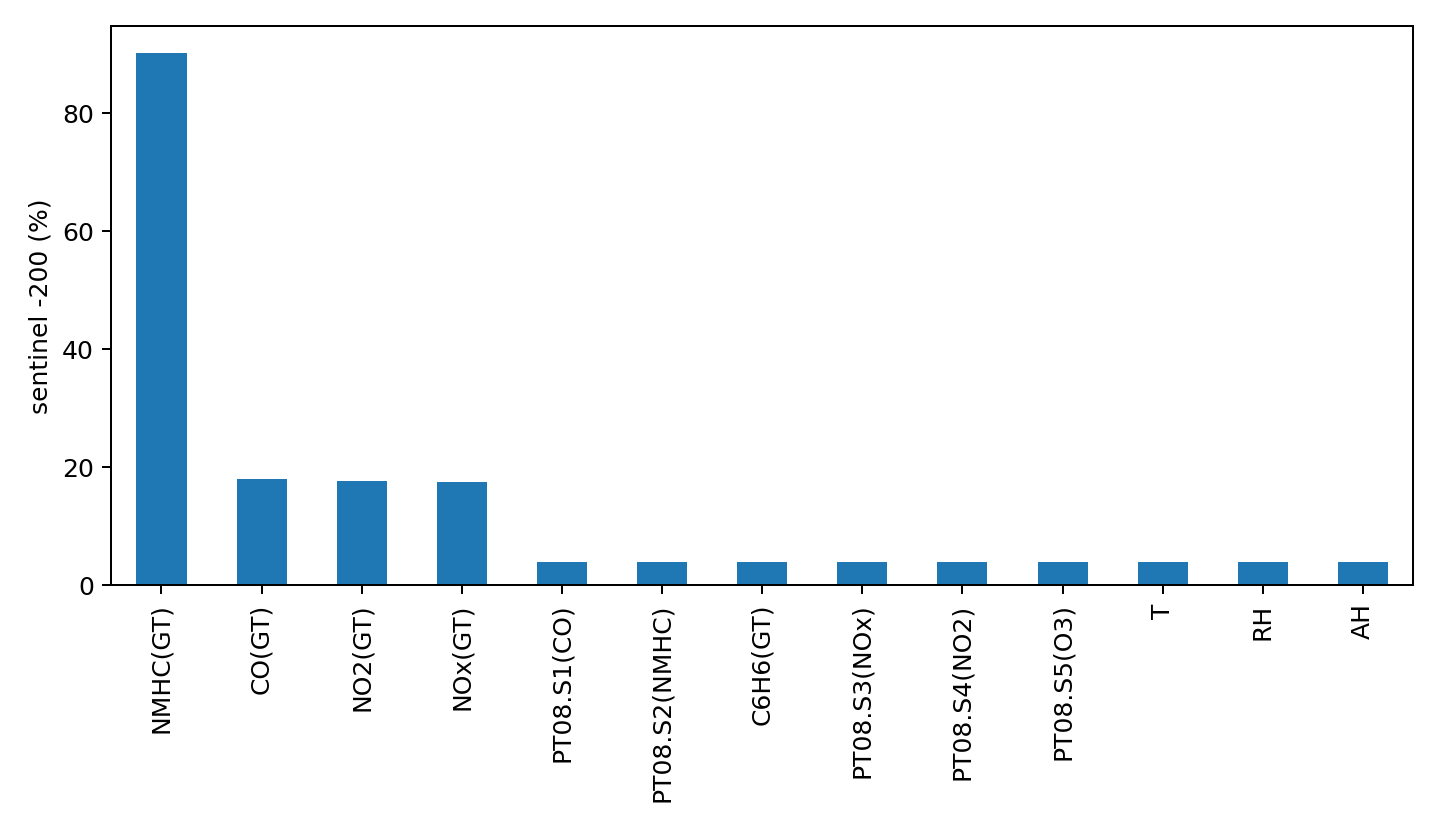
\includegraphics[width=.92\linewidth]{figures/p10_missingness_by_channel.png}
\caption{Fraction of sentinel values by numeric channel in the supplied raw file.}
\end{figure}

\section{Chronological split and restoration rule}
The corpus-reported filtered chronology contains 7,724 transitions divided into 4,634 development, 1,545 re-entry/contact, and 1,545 untouched-future observations. Channel semantics are hidden during representation formation.

Three isolated constructors retain 12 of 13 present-time coordinates. The rejected coordinate is restored only when its inclusion improves actual next-time continuation on successive chronological blocks. The four block increments in correctly predicted future coordinates are
\begin{equation}
158,\quad180,\quad102,\quad121,
\end{equation}
for a total of 561. Exact future vectors improve by 19, 5, 10, and 10 on the four blocks.

\section{Untouched-future result}
After the representation is frozen, the untouched future gives
\begin{table}[H]\centering
\caption{Future performance before and after restoration.}
\begin{tabular}{lrr}
\toprule
metric & 12 channels & 13 channels\\\midrule
coordinate accuracy & 72.0836\% & 74.7125\%\\
exact next vector & 3.7540\% & 7.2492\%\\
\bottomrule
\end{tabular}
\end{table}
The restored representation returns exactly to the independently computed all-channel baseline on both metrics.

\begin{figure}[H]\centering
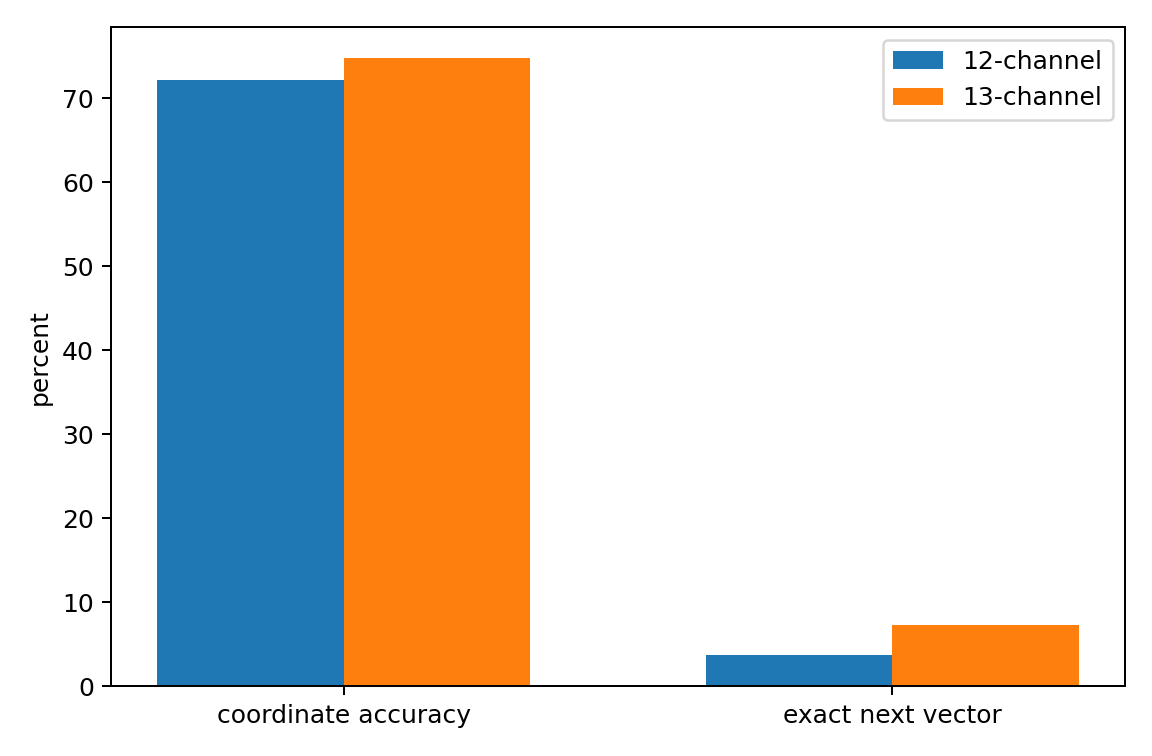
\includegraphics[width=.72\linewidth]{figures/p10_restoration_metrics.png}
\caption{Untouched-future improvement after restoring the omitted channel.}
\end{figure}

A deeper history coordinate selected on contact data is rejected because it worsens both untouched-future objectives. The method therefore supports selective restoration, not indiscriminate state growth.

\section{Leakage and uncertainty requirements}
A clean independent replication requires:
\begin{enumerate}
\item exact static dataset and case identifiers;
\item all coordinate masks and representation constructors;
\item raw-to-7,724 preprocessing code;
\item quantization thresholds and random seeds;
\item row-level predictions;
\item frozen chronology and contact decisions;
\item paired block-bootstrap or permutation intervals preserving serial dependence;
\item modern baselines selected only on development/contact data.
\end{enumerate}
The raw environmental file is included in the ancillary archive. The static 1,797-sample corpus and original constructors are not present in the supplied local files; their numerical results are therefore source-reported rather than independently replayed here.

\section{Interpretation}
The common empirical result is narrow and precise: present compression can erase a relation or coordinate that remains relevant to later continuation. In Study I the retained object is relation among representations; in Study II it is one temporal channel. Neither study proves an asymptotic recurrence exponent without an independently specified repeated residual dynamics.


\section{Complete data and metric separation}
The static study uses a fixed corpus of 1,797 samples and 64 output coordinates. Three representation-specific exact whole-object rates on the untouched 270-case set are
\begin{equation}
92.96\%,\qquad90.74\%,\qquad91.48\%.
\end{equation}
A relation model observes only child status, agreement/disagreement, and frozen contact performance. It reaches
\begin{equation}
\boxed{264/270=97.78\%},
\end{equation}
equal to the empirical oracle ceiling of the available children. Removing the agreement relation creates one additional failure and two additional unknowns. A higher-arity constructor solved none of the six cases where all children failed, so more relation arity is not treated as automatic rescue.

The contextual-output experiment asks a different question: which output coordinates are warranted before values are compared? Its mean return size is 7.985 of 8, admitted-coordinate accuracy is 99.768\%, and whole-return correctness is 98.52\%. These values are never pooled with the 97.78\% whole-object routing result.

\section{Environmental chronology and raw audit}
The supplied semicolon-delimited record contains
\begin{center}
\begin{tabular}{lr}
\toprule
raw rows&9471\\
blank trailer rows&114\\
nonblank hourly rows&9357\\
completely empty columns&2\\
numeric channels&13\\
missing sentinel cells $(-200)$&16701\\
rows complete on all channels&827\\
\bottomrule
\end{tabular}
\end{center}
The nonblank timestamps form a strict hourly sequence from 10 March 2004 18:00 through 4 April 2005 14:00. The reported filtered chronology contains 7,724 transitions: 4,634 development, 1,545 contact/re-entry, and 1,545 untouched future observations.

\section{Chronological restoration result}
Three isolated constructors retained 12 of 13 present-time channels. The omitted channel was restored only after it improved actual next-time continuation on successive chronological contact blocks. The increments in correctly predicted future coordinates were
\begin{equation}
158,\quad180,\quad102,\quad121,
\end{equation}
for a total of 561. Exact future vectors improved by 19, 5, 10, and 10. The representation was then frozen before opening the untouched final segment.

\begin{table}[H]\centering
\caption{Untouched-future comparison.}
\begin{tabular}{lrr}
\toprule
metric&12 channels&13 channels\\\midrule
coordinate accuracy&72.0836\%&74.7125\%\\
exact next vector&3.7540\%&7.2492\%\\
\bottomrule
\end{tabular}
\end{table}
A deeper history representation selected on contact data was rejected because it worsened both untouched metrics. The method therefore permits deletion as well as promotion.

\section{Baseline and statistical requirements}
A clean external reproduction should compare persistence, seasonal persistence, regularized vector autoregression, tree ensembles, nearest-neighbour analogues, and a modern sequence model. Hyperparameters must be selected only on development and contact segments. Serial dependence requires moving-block bootstrap or another dependence-preserving interval method. Report coordinate-level error, exact-vector accuracy, calibration, missingness sensitivity, compute cost, and the probability that every chronological block favours restoration.

\section{Release protocol and evidence status}
The raw environmental file is included and independently audited. The static corpus, exact constructors, row-level predictions, quantization thresholds, and raw-to-7,724 preprocessing program are required for complete independent reproduction. Until released, the corresponding numerical values remain source-reported results rather than externally reproduced facts. That status does not erase the result; it specifies the next admissible test.

\begin{thebibliography}{99}
\bibitem{uci} S. De Vito et al., Air Quality, UCI Machine Learning Repository, 2008.
\bibitem{breiman} L. Breiman, Stacked regressions, Machine Learning 24 (1996), 49--64.
\bibitem{dietterich} T. G. Dietterich, Ensemble methods in machine learning, Multiple Classifier Systems, 2000.
\bibitem{bergmeir} C. Bergmeir, R. Hyndman, and B. Koo, A note on the validity of cross-validation for evaluating autoregressive time series prediction, Computational Statistics and Data Analysis 120 (2018), 70--83.
\end{thebibliography}
\end{document}
